\chapter{Contexte du projet}

\section{Historique}

Dans le cadre de la formation, notre formatrice \formatise nous a proposer de réaliser un jeux de société qui devra a voir un lien avec la formation encoure de $\sharp$Aveni. C'est une façon a la fois ludique et pédagogique de mettre en pratique les connaissance de tout le monde et de revoir les module vue lors des atelier.


\section{Contexte du Projet}

On nous à proposer de crée un jeu dans le cadre de notre formation $\sharp$Aveni, qui est sous la forme d'un jeux de société type carte. Ce Jeux ludique doit permettre aux utilisateurs (formatrice , stagiaire) de développer et confirmer les connaissances a qui lors de la formation.\\

"Le jeux se présente sous la forme d'un paquet de carte, sur les quel on retrouve l'action et la question sur la face avant et le thème sur le dos de la carte.""Le bute final est de récolter le plus de carte pour gagner la partie."Tout ces différents paramètres relatifs à la jouabilité seront présenter en annexe dans une plus large mesure (Règles du jeu).\\

Le jeu s'intitulera "...".

\section{Objectifs de Création du jeu}

\begin{itemize}
	\item Travail ensemble sur un but commun
	\item Travail et Synthétiser nos connaissance sur la Formation Avenir
	\item Développer des valeurs : respect, autonomie, solidarité entre nous
	\item Développer des comportement favorable l'entraide, l'écoute, l'anticipation et l'esprit d'équipe
	\item Construire la cohésion du groupe, favoriser les interactions entre nous
\end{itemize}

\newpage

\section{Objectifs du jeu}

Actuellement, on c'est qu'il n'existe pas de jeu ou d'outil qui est dans la même optique que notre projet. Si on regarde tout le monde prend des notes ou pas, et quand on demande de faire un résumer de l'atelier il se souvienne plus trop ou il on oublier la moutier des chose. Donc mettre ca sous forma d'un jeux de société peut être une idée de faire des carte rappelle sur des choses de base que l'on doit penser quand on dit "C.V." ou "Lettre de Motivation". Autre que aller chercher dans ces feuilles.\\

Le 1\ier objectifs, c'est que l'on peut voir où les personnes on des lacune sur le thème poser. Est d'améliorais se qui doit être améliorais, pour éviter que des personnes soit mie de coter.\\

Le 2\ieme objectifs, c’est d’améliorer l’entente et la convivialité entre tout les participant du jeux.\\

Le bute 1\ier est de passer un bon moment tout en jouent ensemble et de réviser les connaissances des atelier vue pendant la formation encours. \\

Enfin, le maitre du jeux (formateur) pourra mettre les carte avec les thèmes vue par le groupe dans le paquet pour voire leur niveau.

\section{Acteurs}

Madame \formatise, formatrice a ASCEA de Caen, est l'initiateurs du projet. L'équipe de stagiaire qui est constituer de \stagiaire, concepteur du projet. Ils seront a la fois le client et aussi utilisatrice de ce jeu. Le jeu sera par la suite utiliser dans le cadre de la formation $\sharp$Aveni.\\

Cependant, ils on des besoins différents. Pour la formatrice il faut que le jeu soit ludique et en liens avec la formation. Alors que les stagiaires souhaite que le jeux reste divertissant tout en étant ludique.\\

L'équipe de stagiaire et le formatrice assureront à la fois de la maîtrise de l'ouvrage et la création du jeux.

\newpage
\section{Énoncé du besoin fondamental}

%:-+-+-+- Debut
\begin{figure} [!ht]
	\centering
	% Racine en Bas, développement vers le haut
	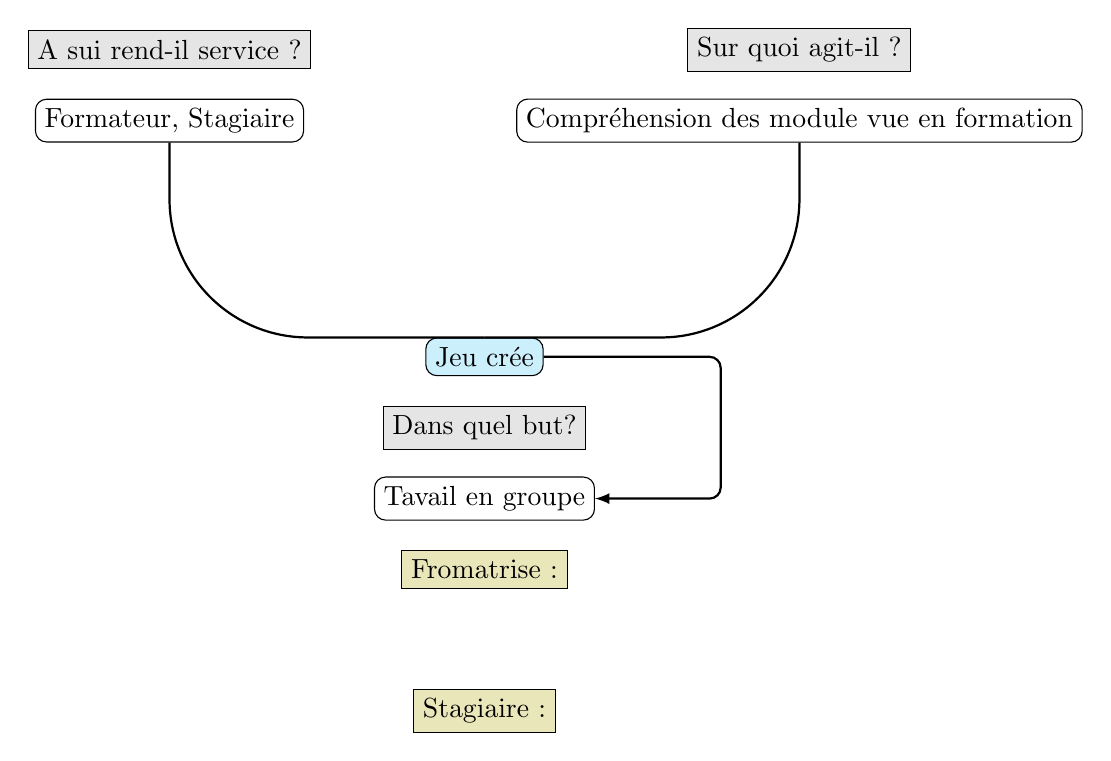
\begin{tikzpicture}[xscale=1,yscale=1]
		% Styles (MODIFIABLES)
		\tikzstyle{corne}=[-,>=latex,thick,rounded corners=50pt]
		\tikzstyle{lienbut}=[->,>=latex,thick,rounded corners=4pt]
		\tikzstyle{but}=[fill=olive!20,draw]
		\tikzstyle{app}=[fill=cyan!20,draw,rounded corners=4pt]
		\tikzstyle{soustete}=[fill=white,draw,rounded corners=4pt]
		\tikzstyle{tete}=[fill=gray!20,draw]
		
		\tikzstyle{etiquette}=[midway,fill=white,draw]
		% Dimensions (MODIFIABLES)
		\def\DistanceInterNiveaux{3}
		\def\DistanceInterFeuilles{2}
		% Dimensions calculées (NON MODIFIABLES)
		\def\NiveauA{(2.3)*\DistanceInterNiveaux}
		\def\NiveauB{(2)*\DistanceInterNiveaux}
		\def\NiveauC{(1)*\DistanceInterNiveaux}
		\def\NiveauD{(0.7)*\DistanceInterNiveaux}
		\def\NiveauG{(0.4)*\DistanceInterNiveaux}
		\def\NiveauE{(0.1)*\DistanceInterNiveaux}
		\def\NiveauF{(-0.5)*\DistanceInterNiveaux}
		
		\def\InterFeuilles{(1)*\DistanceInterFeuilles}
		% Noeuds (MODIFIABLES : Styles et Coefficients d'InterFeuilles)
		\node[tete] (Ta) at ({(-2)*\InterFeuilles},{\NiveauA}) {A sui rend-il service ?};
		\node[soustete] (sTa) at ({(-2)*\InterFeuilles},{\NiveauB}) {Formateur, Stagiaire};
		\node[tete] (Tb) at ({(2)*\InterFeuilles},{\NiveauA}) {Sur quoi agit-il ?};
		\node[soustete] (sTb) at ({(2)*\InterFeuilles},{\NiveauB}) {Compréhension des module vue en formation};
		\node[app] (App) at ({(0)*\InterFeuilles},{\NiveauC}) {Jeu crée};
		\node[tete] (ButT) at ({(0)*\InterFeuilles},{\NiveauD}) {Dans quel but?};	
		\node[soustete] (ButsT) at ({(0)*\InterFeuilles},{\NiveauG}) {Tavail en groupe};	
		\node[but] (ButP) at ({(0)*\InterFeuilles},{\NiveauE}) {Fromatrise :  };
		\node[but] (ButS) at ({(0)*\InterFeuilles},{\NiveauF}) {Stagiaire :  };	
		
		% Arcs (MODIFIABLES : Styles)
		\draw[corne] (App.north)-|(sTa);
		\draw[corne] (App.north)-|(sTb);
		\draw[lienbut] (App.east) --  ({(1.5)*\InterFeuilles},{\NiveauC}) -- ({(1.5)*\InterFeuilles},{\NiveauG}) -- (ButsT.east) ;
		
		
	\end{tikzpicture}
	\caption{Schéma bête a corne du besoins}
\end{figure}
%:-+-+-+-+- Fin

%\begin{figure}
%	\centering
%	\includegraphics[width=0.7\linewidth]{}
%	\caption[courte]{coutee}
%\end{figure}

Résumer du schéma : Le jeu crée permet aux Formateur et Stagiaire de Travail en groupe en travail sur la Compréhension des module vue en formation.\\

Pour le moment, on c'est qu'il n'existe pas de jeu ou d'outil qui peut concurrencer le livrable décrit dans la suite de ce cahier des charges. Les besoins sont bien définis : dans la rubrique Réglé du jeux en annexe. Comme la concurrence est inexistante et que les besoins pouvant être réaliser dans un contexte pédagogique sans empiéter sur l'évolution de la formation. 
